\documentclass[conference]{IEEEtran}
\usepackage{cite}
\usepackage{amsmath,amssymb,amsfonts}
\usepackage{algorithmic}
\usepackage{graphicx}
\usepackage{textcomp}
\usepackage{xcolor}
\usepackage{csquotes}
\usepackage{url}

\def\BibTeX{{\rm B\kern-.05em{\sc i\kern-.025em b}\kern-.08em
    T\kern-.1667em\lower.7ex\hbox{E}\kern-.125emX}}
    
\begin{document}
    %
    %   Title
    %
    \title{Securing Digital Documents with Git: A Novel Approach to Signature Verification\\
    {\footnotesize \textsuperscript{}About the paper titled: “Every Signature is Broken: On the Insecurity of Microsoft Office’s OOXML Signatures.”
    }
    \thanks{}
    }
    %
    %   Authors
    %
    \author{
        \IEEEauthorblockN{1\textsuperscript{st} Tygo van den Hurk}
        \IEEEauthorblockA{\textit{1705709}}
        \textit{t.j.f.h.v.d.hurk@student.tue.nl}
        \and
        \IEEEauthorblockN{2\textsuperscript{st} Aleksandr Bolotskiy}
        \IEEEauthorblockA{\textit{1567209}}
        \textit{a.bolotskiy@student.tue.nl}
        \and
        \IEEEauthorblockN{3\textsuperscript{st} Feiyang Yan}
        \IEEEauthorblockA{\textit{1812076}}
        \textit{f.yan@student.tue.nl}
    }
    \maketitle
    
    %
    %   Abstract
    %
    % \begin{abstract}
    % A brief summary of the issues in this essay (that you write). The abstract should be 100-150 words long. It must summarize what “the essay” contains (and not what the paper contains), including purpose, scope and some very short conclusions. This is the preview of your essay to the reader
    % \end{abstract}
    
    %
    %   Introduction
    %
    \section{Introduction}
        This discussion is based on the paper by Simon Rohlmann, Vladislav Mladenov, Christian Mainka \cite{b1}, which states the insecurity of Microsoft Office’s OOXML signatures. They analyze the structure of office documents and the way digital signatures are verified, and then reveal major discrepancies between them. To visualize the security flaws, they test five attack classes against different Microsoft Office versions on different operating systems and find all tested Office versions are vulnerable.
        
        In recent years, digital transactions play an increasingly important role in the society, making it vital to ensure the integrity and authenticity of digital documents. Therefore, digital signatures started to be widely used. Existing method of digital signature is effective to protect documents and there has been a rapidly growing demand for a working digital signature framework for many fields, including finance and information system departments \cite{b2}, but it is vulnerable to some attacks as shown in recent research \cite{b1} which analyzing vulnerabilities in the signing process of widely-used document formats like word documents.
        
        In consideration of these vulnerabilities, there is a need for innovative approaches to document signing which is able to address these challenges effectively. In this essay, we propose a novel method for signing documents using open-source tools. Our approach takes advantage of the power of Git, a widely adopted version control system. Our approach takes advantage of the power of Git, a widely adopted version control system. By treating each word document as a Git repository and utilizes hash functions to generate signatures \cite{b3}, binding the signatures to the hash values of the documents, we enable a built-in version control which allows users to track changes, revert to previous versions and sign individual commits. This method of digital signature ensures that each change is cryptographically verified and attributed to specific contributors, ensuring the integrity of the document\cite{b4}.
        
        Furthermore, our approach ensures that any changes to the document are signed through Git’s signature validation mechanisms by encoding the document into binary format to match exact saves. Any attempts to modify the document, either by unauthorized party or out of malicious intent, would result in an invalidated signature or the presence of uncommitted changes, which alerts users that there are potential security breaches.
        
        Through this innovative approach, we aim to provide a solution to security problems existed in the process of signing document and verifying signatures shown in the original paper.
    
    %
    %   Main Section A
    %
    \section{Summary}
    %     A couple of main sections: What are the main ideas and results of the paper that you read. These are the things that you will analyze in the discussion section. You are free to use subsections.
    
    % - explain that Microsoft documents are vulnerable
    % - Introduce types of the attacks that document is vulnerable explain how they work and how they bypass signature security
    
    % The main idea of the paper is how Microsoft office has several vulnerabilities, due to flaws in implementation and specification of the file and signature. 
    
    \subsection{File structure flaws}
        OOXML documents consist of a complex structure with multiple interlinked markup and relationship files. These relationship files contain unprotected parts, since signature only works for selected strings. An example is shown \enquote{Thus,
        the body element responsible for the rendered content can
        be defined in other files besides documents.xml, such as
        styles.xml. A distinction whether the inserted content is
        signed or unsigned does not take place and is not distinguishable
        in any way.}.
        
        From these flaws several attack methods were identified:
        \begin{itemize}
            \item  \textbf{Content and Font Injection Attack (CIA):} Because of partial signature it is possible to add reference to a signed OOXML package. One such file people.xml which is processed without reference. Text and Graphics could be added to cover up original content.
            \item  \textbf{Content Masking Attack (CMA):} By removing references to fontTable.xml or style.xml in the document.xml.rels in an unsigned file, attacker can define custom malicious fonts and styles.
            \item  \textbf{Legacy Wrapping Attack (LWA):} When an old binary format is signed by Microsoft office program that uses XML-based signatures it simply creates a valid XML compatable signature. legacy document and signature can be inserted into any OOXML document for a universally valid signature.
        \end{itemize}
    
    \subsection{Implementation flaw}
        Signature value is generated from Signed info, one aspect of which is Package info.
        Package info contains hashes of multiple files that are compared during the signature verification. As it stated by the authors, \enquote{If the reference to
        Package Info is missing, the rendered content of the OOXML
        package is not protected by the signature}. This makes it possible to Forge a Signature on any OOXML document using valid XML signature generated outside Microsoft Word. When forged document is opened Package Info matches existing files, since it is both a generated by an attacker. Signed info is part of the foreign signature so it is validated. Key Info, which is part of a forged document, is shown to the user.
        
        Automatic repair feature in combination with partially signed relationships makes \textbf{ Malicious Repair Attack (MRA)} possible. Making \texttt[Content\_Types].xml in a valid signed document, reference forged information in an unexpected way Automatic repair is triggered. Since the Signed relationships are present and new relationships could be added, file is verified. Automatic repair creates a temporary file displaying fake attacker made content, as long as file wont be saved it will not come up with a warning.
    
    %
    %   Discussion
    %
    \section{Disussion}
    % - Discuss the limitations of the paper and how it is useful is it still an issue
    % - Discuss how git solves these problems how and why (3 points)
    % - ???
    % - Profit
    %
    % this paper is fine, but other did it better
    
    \subsection{Impact and Real-World Implications}
        Microsoft word, or office for that matter arguably one of the most important pieces of software in the word right now. With a current user base of approximately 1.2 billion users worldwide\cite{ms-office-stats}, and an estimated over 500,000 organizations using the this stack for their business makes the security of Office 365 documents is extremely important for the average Joe. One in eight Joe's to be exact. This software having any type of vulnerabilities not something to brush over as any flaws in this system could have huge unseen effects.

        Since the attackers are able to alter signed documents in ways that victims are unaware of, there could be some serious risks associated with the vulnerabilities found. Like for example: fake invoices, fake contracts could be signed and presented as legitimate, fake regulatory and legal documents, or fake academic papers. The extent of this goes as far as the attackers creativity goes.
        
    \subsection{Specific Attack Mechanisms}
        Talking about the flaws in this system. There were 5: Content Injection Attack (CIA), Content Masking Attack (CMA), Legacy Wrapping Attack (LWA), Universal Signature Forgery (USF), Malicious Repair Attack (MRA). In the following sections we'll discuss them briefly.
        
        \subsubsection{Content Injection Attack (CIA): Exploiting standard discrepancies to inject content}
            This attack places malicious content in files intended for metadata, which are not adequately protected by the signature.

        \subsubsection{Content Masking Attack (CMA): Altering the display of content post-signature}
            Here, attackers manipulate styling or font information after the document is signed, altering the displayed content without invalidating the signature.

        \subsubsection{Legacy Wrapping Attack (LWA): Embedding old document signatures in OOXML files}
            This involves embedding a signature from an older document format into an OOXML document, misleading users into trusting the document.
        
        \subsubsection{Universal Signature Forgery (USF): Creating valid-looking signatures from different sources}
            This severe vulnerability allows attackers to use a valid XML signature from another source to create an OOXML document that appears signed and trusted.
        
        \subsubsection{Malicious Repair Attack (MRA): Using the repair functionality to mask malicious content}
            Exploiting the document repair feature in Microsoft Office, this attack hides malicious content until the user triggers a repair process.
        
    \subsection{A better way}
        If there was one thing we learned from reading the paper, and more like it\cite{shadow-attacks} was that partially signed documents are much easier to break. Even signed parts can have references to unsigned parts, leaving an attack surface open where the attacker can change the non-signed parts\cite{PDF-Digital-Signatures-Encryption}. Therefor we suggest a new way of signing and verifying documents using open source methods. Meaning that they are free, and available for any company to implement as they please. We call it signed version controlled documents.
        
        The way it works is by versioning the entire document using Git\cite{git}, then signing each edit (or commit) on a document with GPG keys\cite{gnupg} stored locally on the computer, or submitted by the user. This way, every edit is either signed and the signer is stored in the versioning, or an edit is unsigned and therefor breaks the validity of the document. Since the entire repository is signed with every commit, there would be no way for an attacker to include, or change any files without it being either unsigned, or signed with the wrong key. As every action is commutable with the data from Git. I made a figure to demonstrate the process and inner workings of the concept.
        
        \begin{figure}[h]
          \centering
          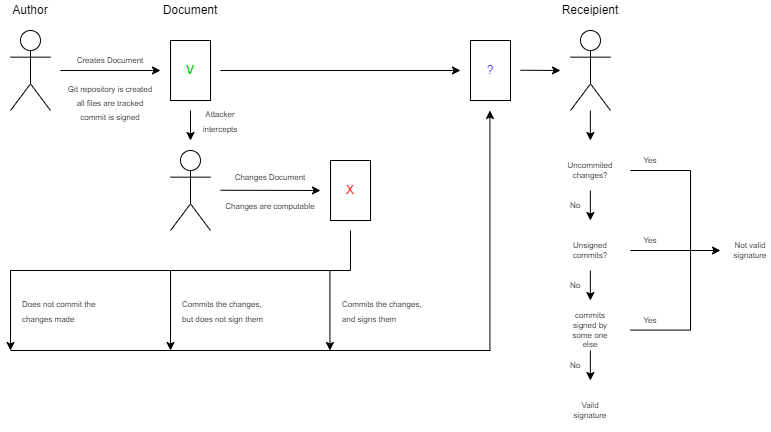
\includegraphics[width=0.5\textwidth]{images/essay.png}
          \caption{How the signage would work.}
          \label{fig:example}
        \end{figure}
        
        The way it works is by hashing the state of the document every time a change is saved. If changes weren't saved, that'd violate the signature. If it was saved but not hashed, that'd violate the signature. If the hash wasn't signed, then that'd violate the signature. if it was signed by the wrong key, that'd violate the signature. This ensures that every change in every version is visible, and signed. 
    
    %
    %   Conclusion
    %
    % \section{Conclusion}
    %      Your group's own opinion on the analyzed material and the judgment of the paper. Be critical. How would you improve it if you were the author/researcher? This has high weight in the assessment.
        
    %
    %   References
    %
    \begin{thebibliography}{00}
        \bibitem{b1} Rohlmann, S., Mladenov, V., Mainka, C., Hirschberger, D., and Schwenk, J., "Every Signature is Broken: On the Insecurity of Microsoft {Office’s} {OOXML} Signatures," in 32nd USENIX Security Symposium (USENIX Security 23), pp. 7411-7428, 2023.
        \bibitem{b2} A. A. Santosa and F. Alamsjah, "The Drivers of a Digital Signature System Adoption: Evidence from Finance and Information System Departments", J. Inf. Syst. Eng. Bus. Intel., vol. 8, no. 1, pp. 80-90, Apr. 2022.
        \bibitem{b3} T. Ozcelebi and J.I. den Hartog, "Lecture Notes: Computer Networks and Security (2IC60)," version 0.7, 2023, Chapter 8, p. 162.
        \bibitem{b4} T. Ozcelebi and J.I. den Hartog, "Lecture Notes: Computer Networks and Security (2IC60)," version 0.7, 2023, Chapter 9: "Cryptography," pp. 176-194.
        
        % Discussion
        \bibitem{shadow-attacks} Christian Mainka, Vladislav Mladenov, and Simon Rohlmann, Shadow Attacks: Hiding and Replacing Content in Signed PDFs, Ruhr University Bochum, \url{https://www.ndss-symposium.org/wp-content/uploads/ndss2021_1B-4_24117_paper.pdf}, 2020.
        \bibitem{PDF-Digital-Signatures-Encryption} PDF Digital Signatures \& Encryption, locklizard, \url{https://www.locklizard.com/document-security-blog/pdf-digital-signatures-encryption/}
        \bibitem{gnupg} The GNU Privacy Guard, Gnu, \url{https://www.gnupg.org/}
        \bibitem{git} Linus Torvalds, Git, Git, \url{https://git-scm.com/about}

        \bibitem{git} Linus Torvalds, Git, Git, \url{https://git-scm.com/about}
        \bibitem{ms-office-stats} Jannik Lindner, Microsoft Office Statistics: Latest Data \& Summary, wifitalents, \url{https://wifitalents.com/statistic/microsoft-office/},  April 23, 2024.

    \end{thebibliography}

\end{document}
